\documentclass[journal]{IEEEtran}
\usepackage{amsmath, amssymb, amsthm}
\usepackage{tikz}
\usetikzlibrary{patterns}
\usetikzlibrary{shapes}

\begin{document}

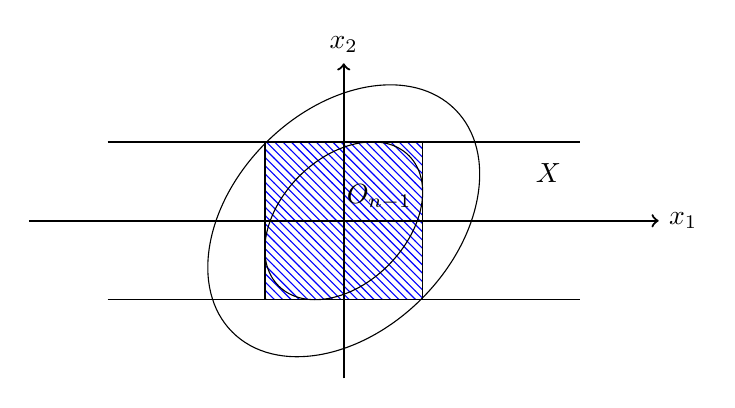
\begin{tikzpicture}
    minimum height = 2cm] at (0,0) {};
\draw[pattern=north west lines, pattern color=blue] (-1,-1) rectangle (1,1);
    \draw[-] (-3,1) -- (3,1);
    \draw[-] (-3,-1) -- (3,-1);
     \draw [rotate=45](0,0) ellipse (1.17cm and 0.8cm);
      \draw [rotate=45](0,0) ellipse (2cm and 1.4cm);
    \draw[thick, ->] (0,-2) -- (0,2) node[above] {$x_2$};
    \draw[thick, ->] (-4,0) -- (4,0) node[right] {$x_1$};
\node at (2.6,0.6) 
    {$X$};
\node at (0.45,0.3) 
    {$O_{n-1}$};
\end{tikzpicture}

\end{document}